Язык программирования Python \cite{python-lang-site} является стандартным выбором языка для разработки и обучения моделей ИНС благодаря богатой экосистеме пакетов. Сами пакеты для разработки моделей ИНС могут быть написаны на более низкоуровневом языке программирования, например, на C++ \cite{cpp-docs} с использованием CUDA \cite{cuda-docs} для высокой производительности кода, в то время как пакет, которым пользуется разработчик, доступен в качестве интерфейса на языке Python для высокой производительности разработчика. Исходя из этого, выбором языка, на котором написаны алгоритмы обработки набора данных DNDD, поиска оптимильных параметров и обучения модели является Python.

\section{ОБРАБОТЧИК НАБОРА ДАННЫХ DNDD}
Обработчик набора данных DNDD доступен как приложение командной строки, полный код которого показан в приложении \ref{app:code}. Параметры обработчика:
\begin{enumerate}
    \item Подмножество игр, которые будут обрабатываться приложением указывается как аргумент командной строки \texttt{--subsets}. Если ведется обработка полного набора данных, то этот аргумент можно опустить или присвоить ему значение \texttt{all}.
    \item Сгенерировать описания неигровых персонажей (далее NPC) можно аргументом \texttt{--generate\_descriptions}. В таком случае необходимо либо иметь доступ к серверу с языковой моделью, либо предварительно запустить сервер самостоятельно, используя например простой интерфейс от Gradio \cite{gradio-docs}. В любом случае желательно передать URL на эндпоинт, где доступна языковая модель, аргументом \texttt{--model\_server\_url}. При отсутствии такого аргумента, URL по умолчанию будет \url{http://127.0.0.1:7860}.
    \item Если список описаний NPC уже есть, то его можно передать в приложение через аргумент \texttt{--description\_file}.
    \item В случае, если требуется, чтобы приложение сохранило работу обработанного набора данных, который готов к конечному использованию для обучения модели, тогда используется аргумент \texttt{--build-final}. Если требуется органичить максимальное количество диалогов NPC, тогда следует использовать аргумент \texttt{--limit\_dialogues}.
\end{enumerate}

При разработке приложения для обработки набора данных DNDD были использованы следующие Python пакеты и библиотеки:
\begin{itemize}
    \item Argparse, встроенная в язык Python библиотека создания программ командной строки.
    \item Tqdm \cite{tqdm-docs} для визуализации прогресса работы приложения.
    \item Requests, встроенная в язык Python библиотека запросов, для доступа к языковой модели через REST <<\textit{Application Programming Interface}>> (API).
    \item Datasets \cite{hf-datasets-docs} для сериализации и хранения обработанного набора данных и объекта, который используется как набор данных при обучении модели.
    \item Transformers \cite{transformers-docs} для оценки количества токенов отправляемых данных в модель для генерации описаний.
    \item Pandas \cite{pandas-docs} для внутренней обработки набора данных.
    \item Os, встроенная в язык Python библиотека взаимодействия с операционной системой, для работы с файлами.
    \item Json, встроенная в язык Python библиотека взаимодействия с JSON файлами, для десериализации исходных данных.
\end{itemize}

\section{МОДУЛИ ОБУЧЕНИЯ И ПОИСКА ОПТИМАЛЬНЫХ ГИПЕРПАРАМЕТРОВ}
Поиск оптимальных гиперпараметров и обучение модели реализованы через Python скрипты. Для обучения модели была использована библиотека Transformers, а для оптимизации процесса обучения и используемых вычислительных мощностей библиотека PEFT \cite{peft-docs}. Для загрузки подготовленных наборов данных используется библиотека Datasets, после чего токенизируется для дальнейшей работы. Для поиска оптимальных гиперпараметров класс sweep библиотеки Weights \& Biases \cite{wandb-docs} перебирает указанный набор.

\section{ДЕМО ПРИЛОЖЕНИЕ ДЛЯ СОЗДАНИЯ ДИАЛОГОВОЙ СИСТЕМЫ ДЛЯ РАЗРАБОТЧИКОВ ВИДЕОИГР}
В качестве тестового приложения диалоговой системы было написано веб-приложение на фреймворке Gradio. В этом приложении можно создать NPC и пообщаться с ним через текстовый или аудио интерфейс. Приложение содержит модули автоматического распознавания речи, эмоциональной классификации речи, классификации намерений, семантического поиска и диалоговой модели. Доступ к приложению осуществляется как через REST API, так и через веб-интерфейс. На экране создания NPC можно заполнить поля, необходимые для описания NPC, и добавить NPC в список доступных для диалога. После создания NPC, на экране диалога можно выбрать конкретного NPC, с которым можно провести диалог. Экран создания NPC можно наблюдать на рис. \ref{demo-npc-creation}, а экран диалога на рис. \ref{demo-dialogue}.
\begin{figure}[H]
    \centering
    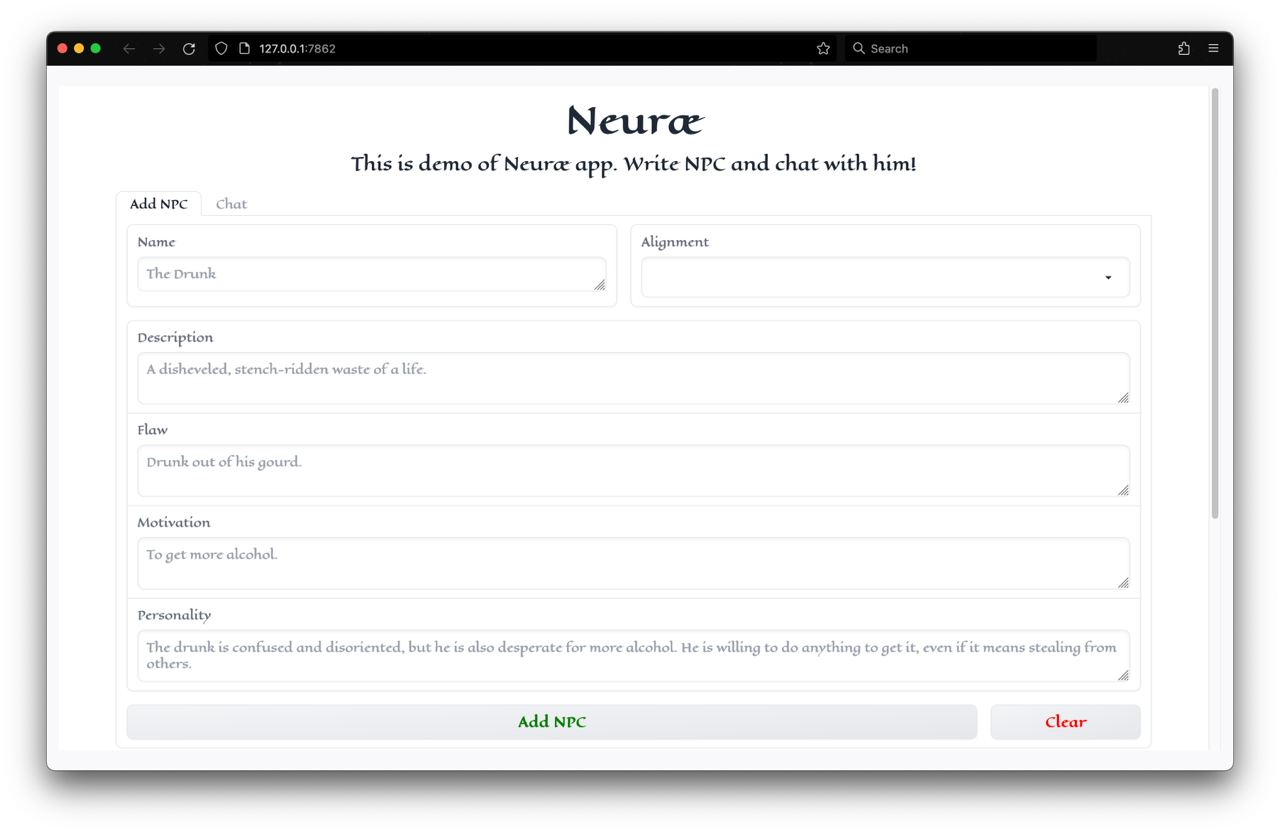
\includegraphics[width=1.\textwidth]{neurae-demo-npc-creation}
    \caption{Экран создания NPC}
    \label{demo-npc-creation}
\end{figure}
\begin{figure}[H]
    \centering
    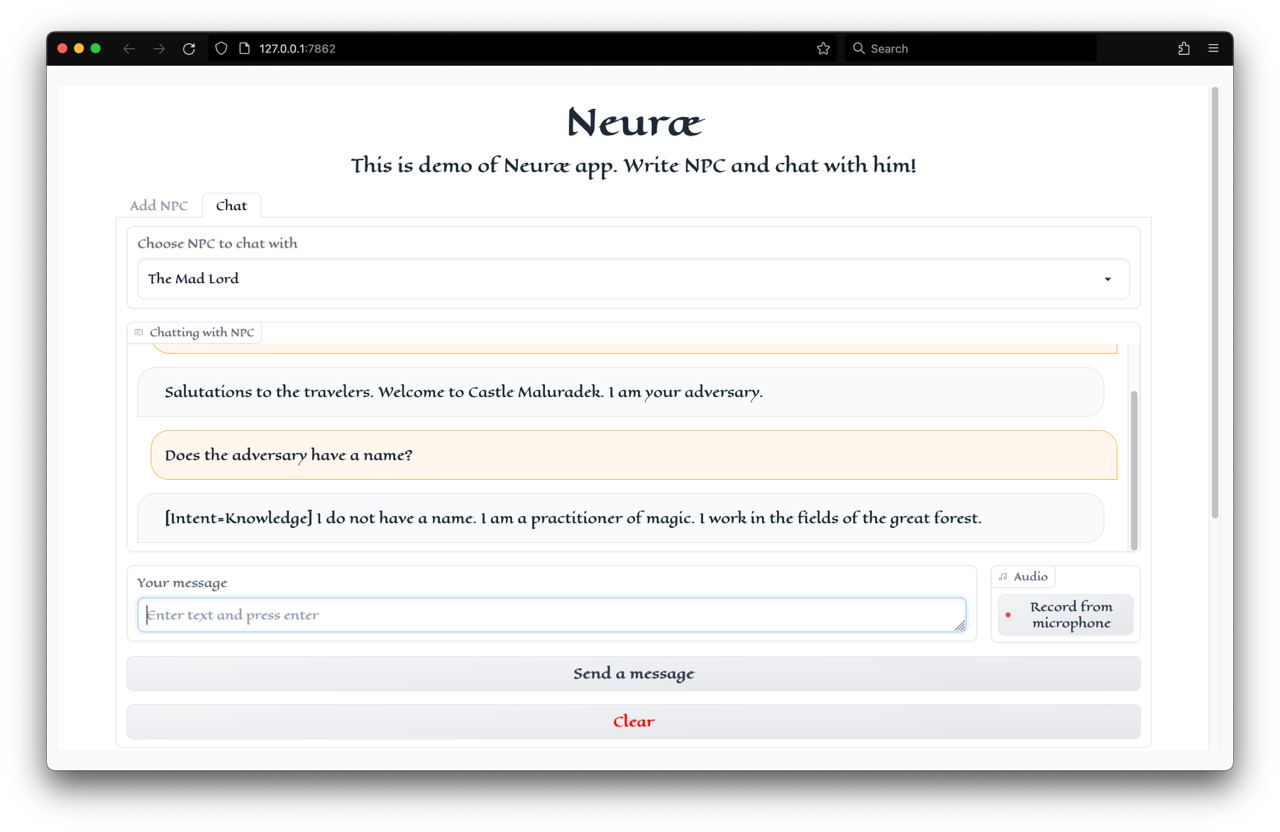
\includegraphics[width=1.\textwidth]{neurae-demo-dialogue}
    \caption{Экран диалога с NPC}
    \label{demo-dialogue}
\end{figure}